%%% retreat document on VBR
\documentclass[review]{acmsiggraph}

%%% Make the ``BibTeX'' word pretty...

\def\BibTeX{{\rm B\kern-.05em{\sc i\kern-.025em b}\kern-.08em
    T\kern-.1667em\lower.7ex\hbox{E}\kern-.125emX}}


\TOGonlineid{XX}

%%% Used by the ``preprint'' variation.
\TOGvolume{0}
\TOGnumber{0}

\title{Uncertainty Modeling for Principled Interactive Image-Based Rendering}

\author{ Rodrigo Ortiz-Cayon and Abdelaziz Djelouah and Michael Goesele and George Drettakis}
\pdfauthor{R. Ortiz-Cayon, A. Djelouah, M. Goesele, G. Drettakis}
%\keywords{radiosity, global illumination, constant time}



%% others
\newcommand{\TODO}[1]{\textcolor{red}{\textbf{#1}}}
\DeclareMathOperator*{\argmin}{\arg\!\min}

\usepackage{comment}

\begin{document}
\maketitle
%%% This is the ``teaser'' command, which puts an figure, centered, below 
%%% the title and author information, and above the body of the content.

 \teaser{
%   \includegraphics[height=1.5in]{images/sampleteaser}
%   \caption{Spring Training 2009, Peoria, AZ.}
 }

\maketitle


%%----------------------------------------------
%% Abstract 
%%
\begin{abstract}

\end{abstract}

%
\copyrightspace

%%----------------------------------------------
%% Introduction 
%%
\section{Introduction}
%\begin{itemize}
%\item Interactive IBR faces challenge of uncertainty in badly reconstructed and unreconstructed regions
%\item Ad-hoc methods, uncertainty not treated in a principled manner, depth synthesis single view, heuristic
%\item Two classes of IBR, forward efficient and high quality (warp), backprojection, handle uncertainty adhoc low quality or are slow.
%\end{itemize}

Recent interactive image-based rendering (IBR) methods allow convincing free-viewpoint navigation
in scenes reconstructed from a small number of images \cite{Eisemann08FT,dibr,chaurasia13,ODD15}.
Despite impressive advances in recent years, these methods are limited in
regions of the scene, which are badly or completely unreconstructed.
Such regions have varying degrees of \emph{uncertainty}, which 
previous solutions treat with heuristic methods: e.g., using dense matching~\cite{dibr}
or heuristic depth synthesis~\cite{chaurasia13}. 
In this paper we propose a principled approach to model uncertainty in IBR, coupled
with a depth synthesis and a IBR algorithm which build on this model.

The idea of modelling uncertainty goes back to the early days of
computer vision~\cite{Szeliski}, but tractable and efficient solutions
have not been developed for interactive IBR. Oversegmentation-based IBR methods achieve
good performance and quality by \emph{forward warping} regions of the image \cite{Zitnick:2004:viewinterp,chaurasia13},
but do not include a measure of uncertainty. Uncertainty has recently
been modeled for more traditional depth-based IBR algorithms \cite{devernay},
which can be considered as derivatives of the Unstructured Lumigraph~\cite{ULR} and use
\emph{backprojection} into the input images. However, the cost of this model is high
and the quality is not always satisfactory, in part because these methods do not use
oversegmentation to preserve depth boundaries.

Our solution addresses these shortcomings by developing a comprehensive model
of uncertainty for IBR. We identify all sources of uncertainty throughout the various processing
stages of modern IBR (calibration, reconstruction, depth synthesis etc.).
We use this model to introduce an iterative multi-view depth synthesis algorithm,
with a Bayesian approach to minimize uncertainty. This preprocessing approach is driven by evaluation of
IBR image quality, and allows fusion of multiple sources of 3D information.
The resulting model of uncertainty 
allows us to develop an IBR algorithm that combines the advantages of  
oversegmentation based forward warping and principled ULR-style backprojection,
notably allowing the use of information from more cameras while maintaining the performance
advantages of forward warping. Finally, we show how to provide plausible 
stereoscopic rendering for regions such as vegetation which can be considered volumetric.

Our contributions are thus:
\begin{itemize}
\item A comprehensive model of uncertainty for interactive IBR.
\item A principled iterative multi-view depth synthesis algorithm, which builds on and informs the uncertainty model.
\item A unified IBR algorithm, which provides a good quality/speed tradeoff by combining the advantages of forward warping and depth-based backprojection algorithms and includes plausible stereoscopic rendering for unreconstructed volumetric regions.
\end{itemize}
Our results show significant improvement over recent algorithms for scenes with poor reconstruction,
allowing the user to move much further from the input viewpoints with the same number of input images.



%% ----------------------------------------------
%% Related work
%%
\section{Related Work}

\begin{itemize}
\item IBR standard text (check OOD15)\cite{Zitnick:2004:viewinterp}
\item Depth synthesis -- check \cite{chaurasia13}
\item Uncertainty modelling -- \cite{devernay} Szeliski, Max etc
\end{itemize}


%% ----------------------------------------------
%% Overview -- needed ?
%%
%\section{Overview}
%\begin{itemize}
\item  A model of uncertainty:
\begin{itemize}
\item reconstruction *(Pujades)
\item depth synthesis
\item depth resynthesis
\item plane estimation
\item compact and efficuient representation
\end{itemize}


\item Iterative multi-view depth synthesis
\begin{itemize}
\item multi-view constraints on depth synthesis (how ?)
\item resynthesis when spixels error is too high in qualeval
\item using alternate sources of depth (objects such as cars, streetview / earth fusion)
\item see also previous notes on depth synthesis
\end{itemize}

\item A new rendering algorithm
\begin{itemize}
\item combines advantages of forward and backward IBR (hierarchical, multi-camera)
\item advantages: many cameras, still very efficient
\item  Optional: good stereo rendering for depth synthesized regions (volumetric rendering)
\end{itemize}
\end{itemize}




%% ----------------------------------------------
%% Uncertainty Model
%%
\section{A Comprehensive Model of Uncertainty}
The IBR processing involves several steps: camera calibration, reconstruction, oversegmentation 
and depth synthesis. 
Each of these steps treats and generates \emph{uncertain data}, possibly coming from multiple sources.
Our goal is to define a model for this uncertainty that will be used to provide a principled
IBR algorithm.

In this work, we chose to consider the first two purely computer vision steps,
i.e., camera calibration and reconstruction, as given. Our model will build on the
data these steps provide, but will not affect these algorithms. The main reason
for this is that calibration and reconstruction often have goals other than image
rendering, e.g., modelling, measurements, fabrication etc. In contrast all subsequent
steps for IBR, e.g., depth synthesis \cite{chaurasia13}, or Bayesian algorithm
labels \cite{ODD15} are specifically targeted to rendering. Consequently
we propose new solutions for these steps, which are tightly integrated with
our uncertainty model.

We will model uncertainty of various quantities used in IBR, namely 3D reconstructed points,
superpixels\cite{slic12}, synthesized depth \cite{chaurasia13} and estimated planes ~\cite{ODD15},
including the influence of each quantity on each other.
\begin{comment}
Or a abstract model that includes the effect of all uncertainties. 
\end{comment}

For 3D reconstructed points we will use the estimation of an ``uncertainty volume''
around the reconstructed parts of the scene, following~\cite{devernay}.
\TODO{give some detail}

For superpixels, we will evaluate how well the oversegmentation algorithm has captured
depth. Even though this oversegmentation is a general approach, our quality criteria
for superpixels are specifically guided by rendering quality. 
\TODO{Possible measures of quality involve uniformity of depth in a superpixel,
some measure of compactness. Other ?}
 
For depth synthesis and plane estimation quality, we will then use ``leave-one-out'' 
quality evaluation~\cite{ODD15}, during
our iterative multi-view depth synthesis (see Sec.~\ref{sec:synth}).
We define the model here, noting the quantities which are iteratively
updated during depth synthesis. \TODO{do this}

The representation is compact and efficient. \TODO{Will be developed iteratively as
the method becomes more precise.}

%\begin{itemize}
%\item reconstruction *(Pujades)
%\item depth synthesis
%\item depth resynthesis
%\item plane estimation
%\item compact and efficuient representation
%\end{itemize}



%% ----------------------------------------------
%% Multi-view Depth
%%
\section{Iterative Multi-View Depth Synthesis \label{sec:synth}}
\subsection{Iterative Multi-View Depth Synthesis}

\TODO{Make this sound less incremental w.r.t \cite{ODD15} and \cite{chaurasia13}}

Previous depth synthesis for IBR ~\cite{chaurasia13} was performed individually for each input image;
while this can give good results in some cases, in many others the depth assigned to superpixels
is inconsistent between views. This results in large popping artifacts when the algorithm blends
from one view to another and in ghosting when inconsistent superpixels are blended.
\TODO{image showing latter}

Synthesizing multi-view consistent depth is not easy: by definition, the superpixels we need
to treat in each input view are not linked in any way, since no -- by construction -- they do not
have any depth.

We will pursue the following ideas to solve this problem:
\begin{enumerate}
\item We will create neighborhood graphs around the superpixels to be matched in each view, and perform graph-matching between views using MVS constraints in the nodes (superpixels) in the graph that do have reconstruction. We can combine this matching with appearance matching (textons or some other measure), which will give a \emph{percentage match} (in most cases only \emph{part} of the pixels will be shared between any two superpixels). Depth synthesis will be performed in an iterative multi-scale approach. Depth will initialize with per-view depth synthesis, and then links between superpixels in other views will be created. An energy minimization problem will be defined, leading to the solution which has lowest error.
Quality (error) will be evaluated using the leave-one-out approach of \cite{ODD15}; depth will be updated during the optimization. The plane estimation step will be included before the quality is evaluated.
\item Inconsistent depth is manifested by abrupt jumps in position of the superpixels corresponding to the same part of an object. Using the matching method above, we will define quality evaluation in time, by moving in paths away from view interpolation, and identifying cases when ``similar'' superpixels move abruptly when switching from one view to another. A (probably) reliable way of doing this is to measure displacement of 3D points, weighted by similarity. This quality metric could directly integrated into the optimization described above.
\end{enumerate}

During each iteration, the uncertainty of the depth synthesis, planar estimation and possibly also the superpixels will be updated, allowing better quality IBR.

\subsection{Using multiple depth sources}

For any given superpixel, depth is assigned directly using the 3D from 
a given reconstruction algorithm, with depth synthesis~\cite{chaurasia13} or
using plane estimation on the point cloud~\cite{ODD15}. Using the coupled synthesis and quality
estimation above, we can also inject other sources of geometry; the quality
of this 3D is then directly evaluated using the ``leave-one-out'' quality estimation
approach~\cite{ODD15}.

A first such source of 3D comes from the improvement in quality in the mesh extraction phase 
of reconstruction algorithms such as \cite{jancosek2011multi,keriven}. 
These algorithms are able to ``stretch'' a smooth surface even in regions with sparse or
poor reconstruction. 

Another source of data includes Google Earth or Bing satelitte reconstructions, which are particularly useful when treating very wide baselines which often cannot be treated well by camera calibration and MVS
reconstruction. This is the case for example for views
one can extract from Google Streetview. 

Both sources of 3D can be directly used in the quality estimation step for each superpixel in the
integrated depth-synthesis/quality evaluation algorithm described above.

%%Iterative multi-view depth synthesis
%\begin{itemize}
%\item multi-view constraints on depth synthesis (how ?)
%\item resynthesis when spixels error is too high in qualeval
%\item using alternate sources of depth (objects such as cars, streetview / earth fusion)
%\item see also previous notes on depth synthesis
%\item motion quality eval
%\item graph matching
%\item iterative approach mixing qual eval and depth synth
%\end{itemize}



%% ----------------------------------------------
%% Unified IBR 
%%
\section{Unified uncertainty aware IBR Algorithm}

%A new rendering algorithm
%\begin{itemize}
%\item combines advantages of forward and backward IBR (hierarchical, multi-camera)
%\item advantages: many cameras, still very efficient
%\item Use uncertainty to maximize render quality. 
%\item Optional: good stereo rendering for depth synthesized regions (volumetric rendering)
%\end{itemize}

Our rendering algorithm consists of three stages, which are closely coupled:
appearance selection (or camera/view selection), 
appearance mapping (warp/backprojection) and appearance synthesis (blending). 
An important requirement throughout this process is the preservation 
of depth contours and depth relationships in the scene.
%In all these steps, the IBR algorithm should preser contours-depth relationships.
Appearance selection and mapping can be defined at the level of rays, pixels,
local regions or even higher level segments. 
As \cite{Zitnick:2004:viewinterp} demostrated, choosing regions represented by superpixels provides robustness to uncertainty
(of several aspects of the image formation process and calibration
offsets).

Rendering algorithms with forward mapping do not enforce the 
\textbf{\emph{continuity}}
property of the novel view \cite{ULR}, since they 
result in popping and produce incomplete regions when the subset
of selected cameras changes.
%producing jumps and
%in-completions when the subset of selected cameras changes. 
To favor speed, forward algorithms select cameras based on spatial proximity with no warranty
of coverage. 
%Popping, spatial discontinuities and incompleteness are common artifacts found in these methods. 
On the other hand, backprojection methods %need an invertible transformation
%or they 
rely completely on the reconstructed geometry to look up source appearance
for the novel view or require some form of dense correspondence~\cite{dibr}. 
The novel view is completed continuously, but only in 
regions where some geometry or correspondences with input images exists. \TODO{mnention that color is interpolated?}. 

In our unified algorithm new views are synthesized by first using 
backprojection for appearance selection at the level of local regions, 
then using forward warping for appearance mapping and finally
blending based on our uncertainty model.
%We formulate the problem of render a novel view as a backward search
%(appearance selection) for a forward mapping (appearance mapping)
%followed for a blending counting for uncertainty (appearance synthesis). 

\begin{figure}[t]
	%\vspace{0.1in}
	\centering
	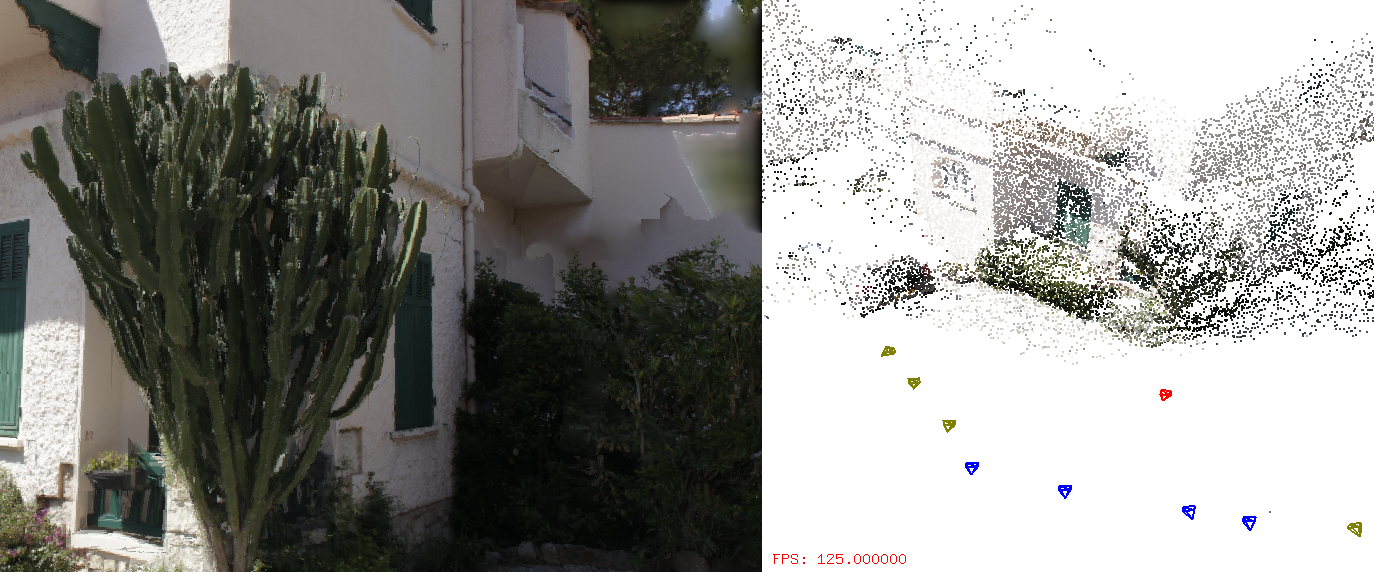
\includegraphics[scale=0.22]{graphics/cam_selection_problem_1.png}
	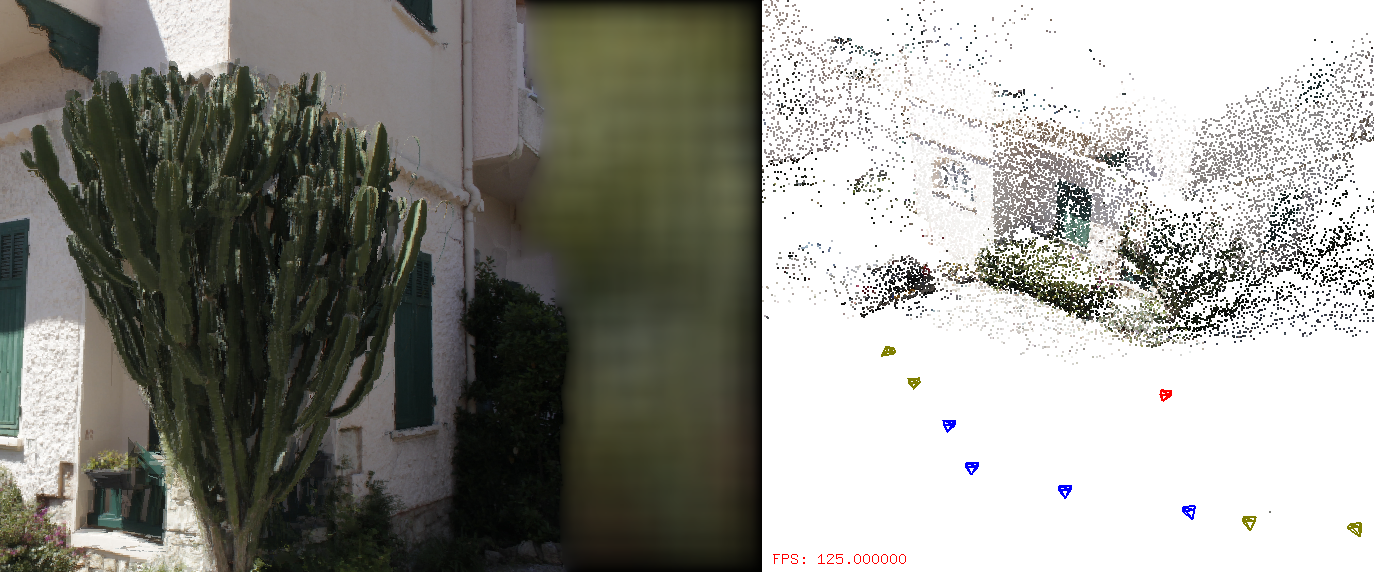
\includegraphics[scale=0.22]{graphics/cam_selection_problem_2.png}	
	\caption{\label{fig:cam_select_problem} 
		Camera selection problem of forward mapping: On the right, we show the input viewpoints (in green), the selected viewpoints (in blue) and the novel viewpoint. Upper row: a novel image generated from the point of view in red. Lower row: the view point has changed one unit w.r.t. the upper row. A discontinuity apprears on the right of the image.}
\end{figure}


\subsection{Appearance Selection:}

%The backward search tries 
We first find regions $S^{i}$ of input camera $C_{i}$
to be used in a further forward mapping and synthesis of a novel view,
using backprojection.
Each region is denoted with $s_{j}^{i}$, where $S^{i}=\{s_{j}^{i}\}$.
Process:
\begin{enumerate}
	\item Overlay a regular grid on the viewport of the novel camera. Cells of the grid are spaced $m$ pixels.
	\item Render a depth map and uncertainty on the novel view.
	\item The depth and uncertainty associated to each vertex of the grid are
	used to look up $s_{j}^{i}$ in each $C_{i}$. The bigger the uncertainty,
	the more chances to hit more than one superpixel $s_{j}^{i}$ in
	$C_{i}$ \TODO{()can be also a function of the contour of superpixel)}.
	\item Create $S^{i}$ as $\cup_j s_{j}^{i}$ in $C_{i}$ assigned to vertices of the grid.
\end{enumerate}
%The expected number of pixels inside of a superpixels is $n^{2}$
%where: $n^{2}=width*height/number\_superpixels$ (see fig). Then $m=(1-\alpha)*n^{2}$,
%where $\alpha$ is the expected overlapping percentage of the transformed superpixels.

\begin{figure}[t]
	%\vspace{0.1in}
	\centering
	
\includegraphics[scale=0.25]{graphics/spixels_overlap.png}
	\caption{\label{fig:spixel_overlaping} 
	In red, the expected overlaping $\alpha$ of mapped superpixels.}
\end{figure}

The expected number of pixels inside a superpixel is $n^{2}$
where: $n^{2}=w \times h/n_s$ (see fig) where the images has resolution
$w \times h$ and $n_s$ is the number of superpixels. Then $m=(1-\alpha)*n^{2}$,
where $\alpha$ is the expected overlapping percentage of the transformed superpixels.

\subsection{Appearance Mapping}

The list of superpixels collected by the appearance selection step
is forward warped as in ~\cite{ODD15}, using the selected 
rendering algorithm. Since the expected number of superpixels is small,
this approach combines the advantages of backprojection methods,
i.e., using a larger number of cameras and those of oversegmentation-based forward warping approaches, i.e., preservation of depth boundaries and efficient projection (since the total number of superpixels is low).
%to an apparent correct place!


\subsection{Appearance Synthesis (Blending and filtering)}

Our synthesis approach will use our uncertainty model to
achieve the best possible quality.
Uncertainty can be used to determine how many images to blend
(typically one or two), and the corresponding weights to be used.


%% -----------------------------------------------
%% Results
%%
\section{Results}
We will compare to \cite{chaurasia13,ODD15}; we expect to see significant improvement due to
the use of more cameras, overcoming the limitation of the number of cameras used and the 
``fronto-parallel'' superpixel issue. 

We also expect to see significantly better quality for
vegetation (no popping or ghosting). We will also need to compare to \cite{dibr}, although we
doubt the quality will be much better. \TODO{maybe ask them for a non-interpolation path}


%% -----------------------------------------------
%% Conclusions
%%
\section{Conclusions}
\input{sec_conclusions}




%% -----------------------------------------------
%% Bibliography
%%

\bibliographystyle{acmsiggraph}
\bibliography{uncertainIBR}
\end{document}
